
% In an 
% % a program $c$ 
% abstract control flow graph for a program $c$, $\absG(c)$, 
% every 
% vertex corresponds to the unique
% label.
% Specifically,
% The edge is directed, 
% representing an abstract transition 
% between two control locations uniquely decided by the labels. 
% (We refer to control the location and the label to the same thing). The abstract transition is in the form of a set of difference constraints for variables, built from the abstract execution trace of the program. For instance, the edge $(l_1, dc, l_2)$ from $l_1$ to $l_2$,
% represents an abstract transition 
% between two control locations with a set of difference constraints on it.
% In this transition, the command labeled with the second location $l_2$, 
% will be executed after execution of the command with label $l_1$,
% % The abstract transition contains a set of difference constraints for variables, 
% with the difference constraints generated by abstracting the command of the first label. Difference constraint is a set of constraints on the difference between variables and constants, which will be formally introduced when we discuss expression abstraction.
% \wq{The edge in the abstract control flow graph comes from the abstract execution trace of the program. The abstract execution trace, an abstract representation of the execution, consists of a list of abstract transitions. Then, every abstract transition in the abstraction execution trace corresponds to an edge in the abstract control flow graph. In another word, the edge $(l_1, dc, l_2)$ in the abstract control flow graph, represents an abstract transition 
% from $l_1$ to $l_2$, with a set of difference constraints $dc$. Also notice, that the different constraints generated during the abstract transition appear in the edge as an annotation.}

% % over the program's abstract execution 

% Overall, the key point of the abstract execution control flow graph is the construction of the abstract execution trace of a program, which relies on a program abstraction procedure in the following steps:

% \begin{enumerate}
% \item Computing the abstract expression for every assignment command in the program.
% \item Computing the abstract event for every labeled command in the program. Intuitively, this abstract event aims 
% to approximate the event in the program's execution trace.
% \item Constructing the abstract execution trace for a program.
% \end{enumerate} 

% We discuss the vertices and edge of the
% abstract control flow graph for a program $c$, $\absG(c)$.

% Every 
% vertex corresponds to the unique
% label.
% Specifically,
% the vertices of this graph is the set of $c$'s labels with an exit label $l_{ex}$, 
% \[ 
% \absV(c) = labels(c)\cup\{l_{ex}\}
% \]
% % corresponding to a label command in the program.

% % \wq{
% The edge in the abstract control flow graph comes from the abstract execution trace of the program. The abstract execution trace, an abstract representation of the execution, consists of a list of abstract transitions. Then, every abstract transition in the abstraction execution trace corresponds to an edge in the abstract control flow graph. In another word, the edge $(l_1, dc, l_2)$ in the abstract control flow graph, represents an abstract transition 
% from $l_1$ to $l_2$, with a set of difference constraints $dc$. Also notice, the difference constraints generated during the abstract transition appear in the edge as an annotation.
% % }

% % over the program's abstract execution 


% % \wq{
% Overall, the vertices can be easily collected and the key point of construction of the abstract execution control flow graph for a program is the abstract execution trace, which relies on the abstraction of expression and abstract transition (we also call it an abstract event), we will discuss in the following section. To make it easy to understand, an abstract control flow graph is a control flow graph, with difference constraints on every edge.
% % } 

% %
% \paragraph*{Expression Abstraction}

% The expression assigned to the variable on the left hand of the assignment command is abstracted to an abstract value: (adopted from the expression abstraction method in paper \cite{sinn2017complexity}). The abstract value is expressed in the form of Difference constraint, denoted as $DC : \mathcal{VAR} \cup \constdom \to \mathcal{\mathcal{VAR} \times (\mathcal{VAR} \cup \constdom) } \times (\mathbb{Z} \cup \{\infty\})$. $\constdom$ is called the Symbolic Constant defined as $\constdom \triangleq \mathbb{N} \cup \inpvar \cup \{\max{(\dbdom)}\} $, which consists of 
% natural numbers $\mathbb{N}$,
% the program's input variables $\inpvar$ 
% and a constant value $\max(\dbdom)$ for estimating the upper bound of variables which are
% assigned by queries. 

% Give an instance of difference constraint used here,
% $DC(\mathcal{VAR} \cup \constdom) \cup \{\top\}$ represents all the difference constraints over 
% variable and symbolic constants. 
% % The difference constraint $DC$ over $\mathcal{VAR} \cup \constdom$ 
% It is a set of the inequality of form $x \leq y + v$ where $x \in \mathcal{VAR} $, 
% $y \in \mathcal{VAR} \cup \constdom$ and $v \in \mathbb{Z}$. 
% This difference constraint is defined in the same way as
% \cite{sinn2017complexity}. For concise, we use $\dcdom^{\top}$ to represent the $DC(\mathcal{VAR} \cup \constdom) \cup \{\top\}$ .


% We show the expression abstraction $\absexpr : \expr \to \mathcal{VAR} \to DC(\mathcal{VAR} \cup \constdom) \cup \{\top\} $ below.

% % We introduce the following notations and operations first
% % % an expression abstraction method based on the expression abstraction in paper \cite{sinn2017complexity}.
% % \\
% % % is enriched into $\constdom \triangleq \mathbb{N} \cup \inpvar \cup \{\max{(\dbdom)}\} $.
% % T
% % \\

% % represents the set of inequality over all $\mathcal{VAR} \cup \constdom$. 

% % The symbolic constant is enriched into $\constdom \triangleq \mathbb{N} \cup \inpvar \cup \{\max{(\dbdom)}\} $.
% % It consists of 
% % natural number $\mathbb{N}$,
% % The symbolic constants $\inpvar$ (i.e., the set of the program's input variables), 
% % and a constant value $\max(\dbdom)$ for estimating the upper bound of variables which are
% % assigned by queries.
% % \\
% % The symbolic constant is enriched into $\constdom \triangleq \mathbb{N} \cup \inpvar \cup \{\max{(\dbdom)}\} $.
% % \\

% % % $ \absdom: \mathcal{P}(DC(\mathcal{VAR} \cup \constdom) \cup \{\top \})$:
% % \\
% % $\constdom: \mathbb{N} \cup \inpvar \cup \{\max{(\dbdom)}\} $ 
% % The constant 
% % \\
% % % $DC(\mathcal{VAR} \cup \constdom)$ represents the set of inequality over all $\mathcal{VAR} \cup \constdom$.
% % \\

% % \[
% % \begin{array}{ll} 
% % \absexpr(y + c, x) = x' \leq y + c & c \in \mathbb{N} \land y \in (VAR \cup \constdom) \\
% % \absexpr(y - c, x) = x' \leq y - c & c \in \mathbb{N} \land y \in (VAR \cup \constdom) \\
% % \absexpr(v, x) = x' \leq v + 0 & v \in (VAR \cup \constdom) \\
% % \absexpr(\aexpr, x) = x' \leq 0 + \infty & \aexpr \text{ doesn't have any of the forms as above} \\
% % \absexpr(\qexpr, x) = x' \leq 0 + \max(\dbdom) & \qexpr \text{ is a query expression} \\
% % \absexpr(\bexpr, x) = x' \leq 0 + 1 & \bexpr \text{ is a boolean expression} \\
% % \end{array}
% % \]
% \[
% \begin{array}{ll} 
% \absexpr(x - v, x) = x' \leq x - v & x \in \grdvar \land v \in \mathbb{N} \\
% \absexpr(y + v, x) = x' \leq y + v & x \in \grdvar \land v \in \mathbb{Z} \land y \in (\grdvar \cup \constdom) \\
% \absexpr(v, x) = x' \leq v + 0 & x \in \grdvar \land v \in (\grdvar \cup \constdom) \\
% \absexpr(y + v, x) = x' \leq y + v & \\
% \grdvar = \grdvar \cup \{y\} & x \in \grdvar \land v \in \mathbb{Z} \land y \notin (\grdvar \cup \constdom) \\
% \absexpr(\qexpr, x) = x' \leq 0 + \max(\dbdom) & x \in \grdvar \land \qexpr \text{ is a query expression} \\
% \absexpr(\bexpr, x) = x' \leq 0 + 1 & x \in \grdvar \land \bexpr \text{ is a boolean expression} \\
% \absexpr(\expr, x) = x' \leq \infty & x \in \grdvar \land \expr \text{ doesn't have any of the forms as above} \\
% \absexpr(\expr, x) = \top & x \notin \grdvar \\
% \end{array}
% \]
 
% % \wq{ 
% $\grdvar$ is the set of variables used in the guard expression of every while the command in the program $c$. 
% % }. 
% In case 4, if a variable $x$, belonging to the set 
% $\grdvar$ is updated by a variable $y$, which isn't in this set, 
% we add $y$ into the set $\grdvar$ and repeat 
% above procedure until $\grdvar$ and $\absexpr(\expr, x)$ is stabilized. 
% % \wq{I do not understand this sentence:-(}
% \\
% Specifically 
% % understanding the intuition, 
% we handle a 
% % simplified 
% normalized guard expression ($ x > 0$ for $x^l \in \lvar_c$)
% in $\ewhile$, and 
% % \wq{I do not understand this sentence:-(}
% %.
% % \\
% % The counter variables only increase, decrease or reset by expression in the form of arithmetic minus and plus (able to extend to max and min.)
% the counter variables only increase, decrease or reset by 
% % expression in the form of 
% simple arithmetic expression (mainly multiplication, division, minus, and plus (able to extend to max and min)). 
% This is the same as in paper \cite{sinn2017complexity}. 
% \\
% For more complex expression assignments, where the counter reset, or calculated from $\elog$, 
% multiplication or division, and expressions involving multiple variables, the constraint is approximated as the reset of $\infty$.
% \\
% % This simplification \wq{which part do we simplify here?} 
% This approximation strategy
% doesn't affect our analysis results in our examples. It is easy to extend the normalized expression 
% into more complex forms as in \cite{sinn2017complexity}, as well as the 
% counter variable manipulation with more advanced expressions.
% % \\ 
% % The boolean expression in the guard of $\ewhile$ command is normalized into form of $ x > 0$ where $x^l \in \lvar_c$ for some $l$.


% \paragraph{Program Event Abstraction}
% We show the abstract event definition, which is generated when computing its abstract execution trace.

% \begin{defn}[Abstract Event]
% \label{def:abs_event}
% Abstract Event: 
% $\absevent \in $
% $\ldom \times \dcdom^{\top} \times \ldom$
% is a 
% % pair of the abstract initial state and final state.
% triple where the first and third components are labels,
% second component is a constraint from $\dcdom^{\top}$.
% % the third % computed from the program's abstract final and initial state, $\absfinal(c)$ and $\absinit(c)$ with a formal definition and algorithm detail in the appendix.
% % the constraint and the third corresponds to a final state.
% \end{defn}
% Specifically, in an abstract event, 
% the first label corresponds to an initial state, and 
% the second label and the constraint correspond to an abstract final state.
% The abstract initial state is a label from $\ldom$.
% The abstract final state is a pair from $\ldom \times \dcdom^{\top}$, 
% where first component is a label from $\ldom$ and the second component is a constraint from $\dcdom^{\top}$.
% %

% %
% Given a program $c$, its abstract initial state,
% and the set of its abstract final state is computed as follows,
% %
% \[
% \begin{array}{ll}
% \absinit(\clabel{\assign{x}{\expr}}{}^l) & = l \\
% \absinit(\clabel{\assign{x}{\expr}}{}^l) & = l \\
% \absinit(\clabel{\eskip}^{l}) & = l \\
% \absinit(\eif [b]^l \ethen c_1 \eelse c_2) & = l \\
% \absinit(\ewhile [b]^l \edo c) & = l \\
% \absinit(c_1 ; c_2) & = \absinit(c_1) \\
% \end{array}
% \]
% %
% Final State Abstraction: 
% $\absfinal: \cdom \to \mathcal{P}(\ldom \times \dcdom^{\top})$,
% computes the set of Abstract Final State for the command. 
% \[
% \begin{array}{ll}
% \absfinal(\clabel{\assign{x}{\expr}}{}^l) & = \{(l, \absexpr\eapp (\expr, x))\} \\
% \absfinal(\clabel{\assign{x}{\query(\qexpr)}}{}^l) & = \{
% (l, x' \leq 0 + \max(\dbdom) )\} \\
% \absfinal(\clabel{\eskip}^{l}) 
% & = \{(l, \top)\} \\
% \absfinal(\eif [b]^l \ethen c_1 \eelse c_2) & = \absfinal(c_1) \cup \absfinal(c_2) \\
% \absfinal(\ewhile [b]^l \edo c) & = \{(l, \top)\} \\
% \absfinal(c_1 ; c_2) & = \absfinal(c_2) \\
% \end{array}
% \]
% %
% \paragraph{Abstract Execution Trace}
% Now, we extract the abstract execution trace $\absflow(c)$ for a program, which computes the Abstract Execution Trace for the program $c$, as a set of the abstract events $\absevent$.
% %
% \begin{defn}[Abstract Execution Trace]
% \label{def:abs_trace}
% $\absflow \in \cdom \to \mathcal{P}( \ldom \times DC(\mathcal{VAR} \cup \constdom) \cup \{\top\}) \times \ldom )$
% \end{defn}
% %

 
% We now show how to compute the abstract execution trace. 
% For simplicity, we use $\mathcal{P}(\absevent)$ represent the power set of all abstract events, and we have $\absflow(c) \in \mathcal{P}(\absevent)$.
% We first append a skip command with 
% % a symbolic label $l_e$, i.e., $\clabel{\eskip}^{l_e}$ at the end of the program $c$, and compute the $\absflow(c) = \absflow'(c')$ for $c'$, where $c' = c;\clabel{\eskip}^{l_e}$ as follows,
% the exist label $l_{ex}$, i.e., $\clabel{\eskip}^{l_{ex}}$ at the end of the program $c$, 
% and compute the $\absflow(c) = \absflow'(c')$ for $c'$, where $c' = c;\clabel{\eskip}^{l_{ex}}$ as follows,
% %
% {\footnotesize
% \[
% \begin{array}{ll}
% \absflow'(\clabel{\assign{x}{\expr}}{}^l) & = \emptyset \\
% \absflow'(\clabel{\assign{x}{\query(\qexpr)}}{}^l) & = \emptyset \\
% \absflow'([\eskip]^{l}) & = \emptyset \\
% \absflow'(\eif [b]^l \ethen c_t \eelse c_f) & = \absflow'(c_t) \cup \absflow'(c_f)
% % \\ & \quad 
% \cup \{(l, \top, \absinit(c_t) ) , (l, \top, \absinit(c_f)) \} \\
% \absflow'(\ewhile [b]^l \edo c_w) & = \absflow'(c_w) \cup \{(l, \top, \absinit(c_w)) \} 
% % \\ & \quad 
% \cup \{(l', dc, l)| (l', dc) \in \absfinal(c_w) \} \\
% \absflow'(c_1 ; c_2) & = \absflow'(c_1) \cup \absflow'(c_2) 
% % \\ & \quad 
% \cup \{ (l, dc, \absinit(c_2)) | (l, dc) \in \absfinal(c_1) \} \\
% \end{array}
% \]
% }

% Notice $\absflow'([x := \expr]^{l})$, $\absflow'([x := \query(\qexpr)]^{l})$ and $\absflow'([\eskip]^{l})$ are all empty set. 
% For every event $\event$ with label $l$ in an execution trace $\trace$ of program $c$, 
% there is an abstract event in the program's abstract execution trace of form $(l, \_, \_)$. We also show the soundness of the abstract execution trace, which says \wq{...}
% \begin{lem}[Soundness of the Abstract Execution Trace]
% \label{lem:abscfg_sound}
% Given a program ${c}$, we have:
% %
% \[
% \begin{array}{l}
% \forall \vtrace_0, \trace \in \mathcal{T} , \event = (\_, l, \_) \in \eventset \st
% \config{{c}, \trace_0} \to^{*} \config{\eskip, \trace_0 \tracecat \vtrace} 
% \land \event \in \trace 
% \\
% \qquad \implies \exists \absevent = (l, \_, \_) \in (\ldom\times \dcdom^{\top} \times \ldom) \st 
% \absevent \in \absflow(c)
% \end{array}
% \]
% \end{lem}
% % This lemma is proved formally in appendix~\ref{apdx:reachability_soundness}.
% % For every event $\event$ with label $l$ in an execution trace $\trace$ of program $c$, 
% % there is an abstract event in program's abstract execution trace of form $(l, \_, \_)$. 
% This lemma is proved formally in Lemma~\ref{lem:abscfg_sound} in appendix~\ref{apdx:reachability_soundness}.
% \\
% For every labeled variable in program $c$, $x^l \in \lvar_c$, there is a unique abstract event in program's abstract execution trace $\absevent \in \absflow(c)$ of form $(l, \_, \_)$. 
% \begin{lem}[Uniqueness of the Abstract Execution Trace]
% \label{lem:abscfg_unique}
% Given a program ${c}$, we have:
% %
% \[
% \begin{array}{l}
% \forall \vtrace_0, \trace \in \mathcal{T} , \event = (\_, l, \_, \_) \in \eventset^{\asn} \st
% \config{{c}, \trace_0} \to^{*} \config{\eskip, \trace_0 \tracecat \vtrace} 
% \land \event \in \trace 
% \\
% \qquad \implies \exists! \absevent = (l, \_, \_) \in (\ldom\times \dcdom^{\top} \times \ldom) \st 
% \absevent \in \absflow(c)
% \end{array}
% \]
% \end{lem}
% This lemma and proof are also 
% formalized in Lemma~\ref{lem:absevent_unique} in appendix~\ref{apdx:reachability_soundness}.

% Then, we build the edge for $c$'s abstract control flow graph as follows,
% \[
% \absE(c) = \{(l_1, dc, l_2) | (l_1, dc, l_2) \in \absflow(c)\}
% \]

% % We have a pre-processing algorithm to go through the programs and return the list of labels associated with a loop and whose visiting times need to be analyzed.
% %


% \paragraph{Abstract Control Flow Graph} 
% With the vertices $\absV(c)$ and edges $\absE(c)$ ready, we construct the abstract control flow graph, formally 
% % Through a program $c$'s abstract execution trace, its abstract control flow graph is computed 
% defined in 
% Definition~\ref{def:abs_cfg}.
% % Given program $c$ with its abstract control flow $\absflow(c)$, the Abstract Control Flow Graph:
% % \\
% \begin{defn}[Abstract Control Flow Graph]
% \label{def:abs_cfg}
% Given a program $c$, 
% with its abstract control flow $\absflow(c)$
% its abstract control flow graph $\absG(c) =(\absV(c), \absE(c), \absW(c))$ is defined as follows,
% \\
% % \highlight{
% % :
% %
% % \\
% $\absE(c) = \{(l_1, dc, l_2) | (l_1, dc, l_2) \in \absflow(c)\}$,
% \\
% $\absV(c) = labels(c)\cup\{l_{ex}\}$
% \\
% $\absW(c) 
% \triangleq \left\{ (l, w) \in \mathbb{L} \times EXPR(\constdom) \right\}$.
% % }
% % \\
% % , where the weight of every label is to be computed in the next step.
% \end{defn}
% % 
% % The vertices $\absV(c)$ in this graph are program's labels with an exit label $l_{ex}$.
% % Each directed 
% % edge $(l_1, dc, l_2)$ from $l_1$ to $l_2$,
% % represents an abstract transition 
% % between two control locations with a set of difference constraints on it.
% % % , i.e., the labels of two commands (we call the labels also control the location and they refer to the same thing), 
% % % where 
% % In this transition, the command labeled with the second location $l_2$, 
% % will be executed after execution of the command with label $l_1$,
% % % The abstract transition contains a set of difference constraints for variables, 
% % with the difference constraints generated by abstracting the command of the first label.
% % % \\
% % % It is easy to show for every $(l_1, dc, l_2) \in \absflow(c)$ such that $l_2 \neq l_e$, $(l_1, l_2) \in flow(c)$. The formal Lemma and proof can be found in Lemma~\ref{lem:flow_to_absflow} in appendix~\ref{apdx:reachability_soundness}.
% Notice we also define the $\absW(c)$ in this graph without giving an actual value.
% This $\absW(c)$ is the set of weights for every 
% % vertex 
% label. The weight is a symbolic expression over the symbolic constant, 
% which is the estimated upper bound on the number of visiting times for every control location
% through the reachability bound analysis as follows.
%
% It is easy to show for every $(l_1, dc, l_2) \in \absflow(c)$ such that $l_2 \neq l_e$, $(l_1, l_2) \in flow(c)$. The formal Lemma and proof can be found in Lemma~\ref{lem:flow_to_absflow} in appendix~\ref{apdx:reachability_soundness}.
%
In order to analyze the static data dependency relation and the dependency relation quantity,
I first build an abstract control flow graph as the base step for the analysis in Section~\ref{subsubsec:static-datadep}
and Section~\ref{subsubsec:static-reachability} as follows.
\paragraph*{Abstract Control Flow Graph}
I define an abstract control flow graph for program $c$, 
% which mimics the standard control flow graph, 
whose vertices are the unique labels from $c$'s labeled commands with
% . We also have
a special label $ex$ for the exit of the program. Each edge $(l_1, dc, l_2)$ of our abstract control flow graph is annotated with a difference constraint, which is used to describe the execution of $l_1$. The edge itself talks about the transition between $l_1$ to $l_2$. Still for the same $\kw{twoRounds(k)}$ example as overview, its generated abstract control flow graph is shown in Figure~\ref{fig:abscfg_tworound}(b).
For example, the edge $(0, a \leq 0, 1)$ on the top, tells us the command 
$\clabel{\assign{a}{0}}^0$ is executed with next continuation location $1$,
where the 
command $\clabel{\assign{j}{k}}^1$ will be executed next.
The constraint $a \leq 0$ is a difference constraint, generated by abstracting from the assignment command $\assign{a}{0}$,
representing that value of $a$ is less than or equals to $0$ after 
location $0$ before executing the command at line $1$. The difference constraint is an inequality relation. The left-hand side of the inequality talks about variables before the execution and the right-hand side ascribes those after the execution. 
The difference constraint $a < a+x $ on the edge $(5, a < a + x, 2)$ describes the execution of the command $\clabel{\assign{a}{a + x}}^5$.
% Look at the $a < a+x $ on the edge $5$ to $2$, which describes the execution of the command at line $5$, which is an assignment $a = a+x$. The $a$ on the left side of $a < a+x$ represents the value of $a$ after the assignment, while the right-hand side $a$ stores the value before the assignment. 
The cycle $2 \to 4 \to 5 \to 2$ in Figure~\ref{fig:abscfg_tworound}(b). 
Please also look at the edge from $3$ to $4$, which talks about the query. The $x < Q_m$ describes the execution of a query request (the command at line 3), and the query results stored in $x$ are bounded by $Q_m$.
$Q_m$ is the maximal value for query requesting result from the database $DB$. $\top$ means there is no assignment executed, for example, we have the difference constraint $\top$ on the edge $2$ to $6$, which means at line $2$, there is no assignment (it is a testing guard $j>0$.) 
%
\begin{figure} 
\centering
\begin{subfigure}{.2\textwidth}
\begin{centering}
{\small
$
 \begin{array}{l}
 \clabel{ \assign{a}{0}}^{0} ; 
 \clabel{\assign{j}{k} }^{1} ; \\
 \ewhile ~ \clabel{j > 0}^{2} ~ \edo ~ \\
 \Big(
 \clabel{\assign{x}{\query(\chi[j])} }^{3} ; \\
 \clabel{\assign{j}{j-1}}^{4} ;\\
 \clabel{\assign{a}{x + a}}^{5} \Big);\\
 \clabel{\assign{l}{\query(\chi[k]*a)} }^{6}\\
 \end{array}
$
}
\caption{}
\end{centering}
\end{subfigure}
 \begin{subfigure}{.35\textwidth}
 \begin{centering}
% \todo{abstract-cfg for two round}
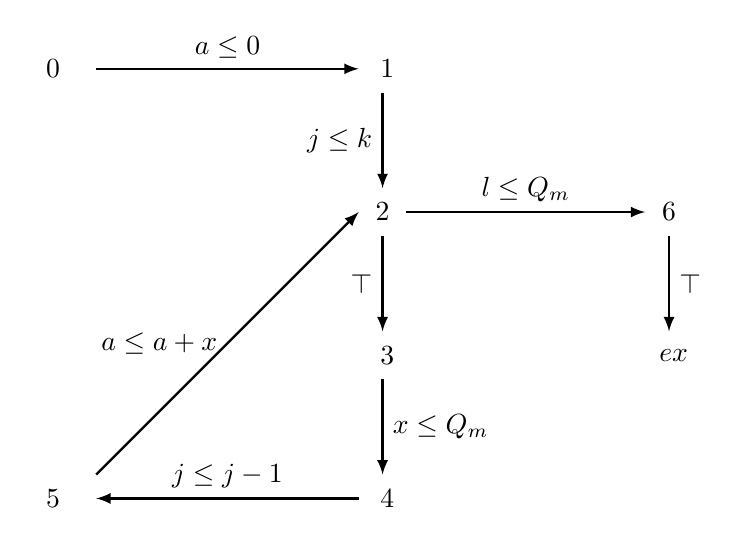
\begin{tikzpicture}[scale=\textwidth/20cm,samples=200]
\draw[] (-7, 10) circle (0pt) node{{ $0$}};
\draw[] (0, 10) circle (0pt) node{{ $1$}};
\draw[] (0, 7) circle (0pt) node{\textbf{$2$}};
\draw[] (0, 4) circle (0pt) node{{ $3$}};
\draw[] (0, 1) circle (0pt) node{{ $4$}};
\draw[] (-7, 1) circle (0pt) node{{ $5$}};
% Counter Variables
\draw[] (6, 7) circle (0pt) node {\textbf{$6$}};
\draw[] (6, 4) circle (0pt) node {{ $ex$}};
%
% Control Flow Edges:
\draw[ thick, -latex] (-6, 10) -- node [above] {$a \leq 0$}(-0.5, 10);
\draw[ thick, -latex] (0, 9.5) -- node [left] {$j \leq k$} (0, 7.5) ;
\draw[ thick, -latex] (0, 6.5) -- node [left] {$\top$} (0, 4.5);
\draw[ thick, -latex] (0, 3.5) -- node [right] {$x \leq Q_m$} (0, 1.5) ;
\draw[ thick, -latex] (-0.5, 1) -- node [above] {$j \leq j - 1$} (-6, 1) ;
\draw[ thick, -latex] (-6, 1.5) -- node [left] {$a \leq a + x$} (-0.5, 7) ;
\draw[ thick, -latex] (0.5, 7) -- node [above] {$l \leq Q_m$} (5.5, 7);
\draw[ thick, -latex] (6, 6.5) -- node [right] {$\top$} (6, 4.5) ;
\end{tikzpicture}
\caption{}
 \end{centering}
 \end{subfigure}
 \begin{subfigure}{.35\textwidth}
 \begin{centering}
 % \todo{abstract-cfg for two round}
 \begin{tikzpicture}[scale=\textwidth/20cm,samples=200]
 \draw[] (-10, 10) circle (0pt) node{{ $0: 1$}};
 \draw[] (0, 10) circle (0pt) node{{ $1: 1$}};
 \draw[] (0, 7) circle (0pt) node{\textbf{$2: k$}};
 \draw[] (0, 4) circle (0pt) node{{ $3: k$}};
 \draw[] (0, 1) circle (0pt) node{{ $4: k$}};
 \draw[] (-10, 1) circle (0pt) node{{ $5: k$}};
 % Counter Variables
 \draw[] (6, 7) circle (0pt) node {\textbf{$6: 1$}};
 \draw[] (6, 4) circle (0pt) node {{ $ex: 1$}};
 %
 % Control Flow Edges:
\draw[ thick, -latex] (-8, 10) -- node [above] {$a \leq 0$}(-1.5, 10);
\draw[ thick, -latex] (0, 9.5) -- node [left] {$j \leq k$} (0, 7.5) ;
\draw[ thick, -latex] (0, 6.5) -- node [left] {$\top$} (0, 4.5);
\draw[ thick, -latex] (0, 3.5) -- node [right] {$x \leq Q_m$} (0, 1.5) ;
\draw[ thick, -latex] (-1.5, 1) -- node [above] {$j \leq j - 1$} (-8, 1) ;
\draw[ thick, -latex] (-8, 1.5) -- node [left] {$a \leq a + x$} (-1.5, 7) ;
\draw[ thick, -latex] (1.5, 7) -- node [above] {$l \leq Q_m$} (4.5, 7);
\draw[ thick, -latex] (6, 6.5) -- node [right] {$\top$} (6, 4.5) ;
 \end{tikzpicture}
 \caption{}
 \end{centering}
 \end{subfigure}
% \begin{subfigure}{.3\textwidth}
% \begin{centering}
% \begin{tikzpicture}[scale=\textwidth/18cm,samples=200]
% \draw[] (0, 10) circle (0pt) node
% {{ $a^0: {}^1_{0}$}};
% \draw[] (0, 7) circle (0pt) node
% {\textbf{$x^3: {}^{k}_{1}$}};
% \draw[] (0, 4) circle (0pt) node
% {{ $a^5: {}^{k}_{0}$}};
% \draw[] (0, 1) circle (0pt) node
% {{ $l^6: {}^{1}_{1}$}};
% % Counter Variables
% \draw[] (5, 9) circle (0pt) node {\textbf{$j^2: {}^{1}_{0}$}};
% \draw[] (5, 6) circle (0pt) node {{ $j^4: {}^{k}_{0}$}};
% %
% % Value Dependency Edges:
% \draw[ ultra thick, -latex, densely dotted,] (0, 1.5) -- (0, 3.5) ;
% \draw[ ultra thick, -latex, densely dotted,] (0, 4.5) -- (0, 6.5) ;
% \draw[ thick, -latex] (0, 7.5) -- (0, 9.5) ;
% \draw[ thick, -Straight Barb] (1.5, 3.5) arc (120:-200:1);
% \draw[ thick, -Straight Barb] (6.5, 6.5) arc (150:-150:1);
% \draw[ thick, -latex] (5, 6.5) -- (5, 8.5) ;
% % Control Dependency
% \draw[ thick,-latex] (1.5, 7) -- (4, 9) ;
% \draw[ thick,-latex] (1.5, 4) -- (4, 9) ;
% \draw[ thick,-latex] (1.5, 7) -- (4, 6) ;
% \draw[ thick,-latex] (1.5, 4) -- (4, 6) ;
% \end{tikzpicture}
% \caption{}
% \end{centering}
% \end{subfigure}
 \vspace{-0.3cm}
 \caption{
 (a) The same $\kw{towRounds(k)}$ program as Figure~\ref{fig:twoRounds_example}
 (b) The abstract control flow graph for $\kw{towRounds(k)}$ 
 (c) The abstract control flow graph with the reachability bound for $\kw{towRounds(k)}$.}
 \vspace{-0.5cm}
 \label{fig:abscfg_tworound}
\end{figure}
%

